
\documentclass[aspectratio=169]{beamer}
\usetheme{metropolis}           % Use metropolis theme
\usepackage[utf8]{inputenc}
\usepackage{graphicx}
\usepackage{eso-pic}
\usepackage{graphics}
\usepackage{tikz}
\usepackage[export]{adjustbox}
\usepackage{multicol}
\usepackage{listings}
\usepackage{helvet}
\usepackage{booktabs}
\usepackage{threeparttable}


\title{Descriptive Statistics: \newline Creating Tables}
\date{\today}
\author{Benjamin Daniels} % Name of author(s) of session here
\institute{Development Impact Evaluation (DIME) \newline The World Bank }
\setbeamercolor{background canvas}{bg=white}	% Sets background color

% The below command places the World Bank logo and DIME logo to the right corner
\titlegraphic{%
	\begin{picture}(0,0)
	\put(330,-180){\makebox(0,0)[rt]{
\includegraphics[width=3cm]{img/WB_logo}}}
	\end{picture}%
	\begin{picture}(0,0)
	\put(390,-180){\makebox(0,0)[rt]{
\includegraphics[width=1.5cm]{img/i2i}}}
	\end{picture}%
}

%%% Section page with picture of Light bulb
\makeatletter
\defbeamertemplate*{section page}{mytheme}[1][]{
	\centering
	\begin{minipage}{22em}
		\raggedright
		\usebeamercolor[fg]{section title}
		\usebeamerfont{section title}
		\par
		\ifx\insertsubsectionhead\@empty\else%
		\usebeamercolor[fg]{subsection title}%
		\usebeamerfont{subsection title}%
		\fi
		\ifstrempty{#1}{}{%
			\includegraphics[width=100mm, height=60mm]{#1}%
		}
		\insertsectionhead\\[-1ex]
		\insertsubsectionhead
		\usebeamertemplate*{progress bar in section page}
		
	\end{minipage}
	\par
	\vspace{\baselineskip}
}
\makeatother

%%% Define a command to include picture in section, 
%%% make section, and revert to old template
\newcommand{\sectionpic}[2]{
	\setbeamertemplate{section page}[mytheme][#2]
	\section{#1}
	\setbeamertemplate{section page}[mytheme]
}

%%% The command below allows for the text that contains Stata code
\lstset{ %
	backgroundcolor=\color{white},
	basicstyle=\tiny,
	breakatwhitespace=false,
	breaklines=true,
	captionpos=b,
	commentstyle=\color{green},
	escapeinside={\%*}{*)},
	extendedchars=true,
	frame=single,
	numbers=left,
	numbersep=5pt,
	numberstyle=\tiny\color{gray},
	rulecolor=\color{black},
	showspaces=false,
	showstringspaces=false,
	showtabs=false,
	stringstyle=\color{mauve},
	tabsize=2,
	title=\lstname,
	morekeywords={not,\},\{,preconditions,effects },
	deletekeywords={time}
}

%% The below command creates the ligh bulb logos in the top right corner of the 
\begin{document}
	
{
	\usebackgroundtemplate{
\includegraphics[height=55mm, right]{img/top_right_corner.pdf}}
	\maketitle
}

\begin{frame}{What are descriptive statistics?}
\begin{multicols}{2}	

\begin{itemize}[<default overlay specification>]
	\item<1> Numbers or figures that paint a picture of what a given dataset looks like. 
	\item<1> They begin to help us understand the important features of our dataset, and can be useful in directing us towards areas of further analysis.
	\item<1> We will also show how to make basic regression outputs. 
\end{itemize}

\begin{figure}
	\centering
	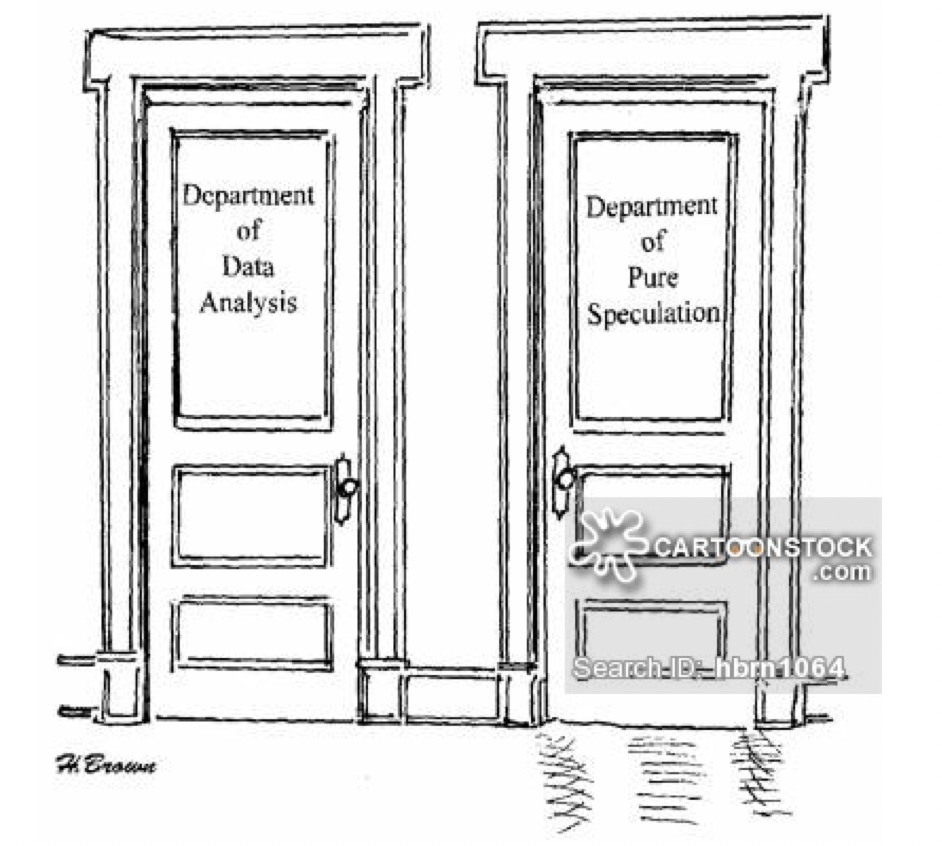
\includegraphics[width=60mm]{img/Descriptives}
\end{figure}

\end{multicols}
\end{frame}


\begin{frame}{Descriptive statistics are NOT regressions}
	\begin{multicols}{2}	
		
		\begin{itemize}[<default overlay specification>]
			\item<1> This is “Anscombe’s Quartet.”
			\item<1> Every set here has:
					\newline - The same means (x and y).
					\newline - The same variances (x and y). 
					\newline - The same correlation coefficient.
					\newline - The same regression coefficient.
					\newline - The same regression R2.
			\item<1> Regression analysis tells you nothing about the world if you don’t understand the shape of the world you are in!
		\end{itemize}
		
		\begin{figure}
			\centering
			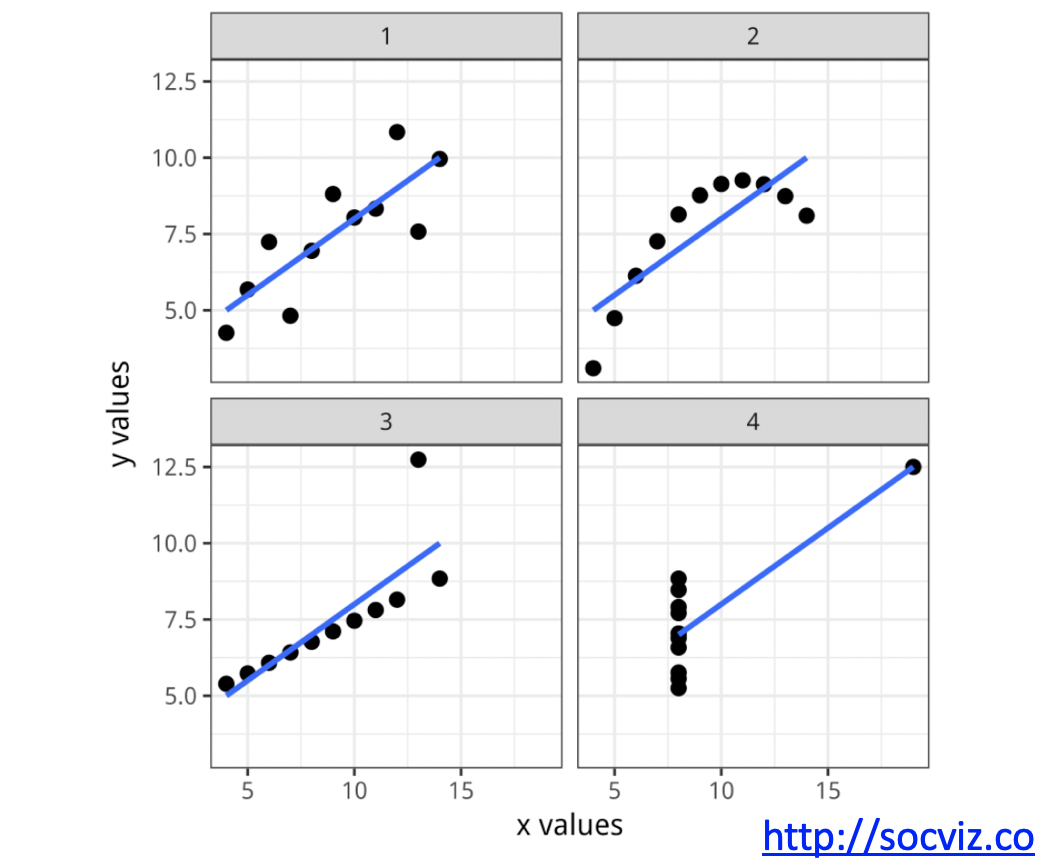
\includegraphics[width=60mm]{img/Regressions}
		\end{figure}
		
	\end{multicols}
\end{frame}


\begin{frame}{Data can take almost any shape}
	
\begin{figure}
	\centering
	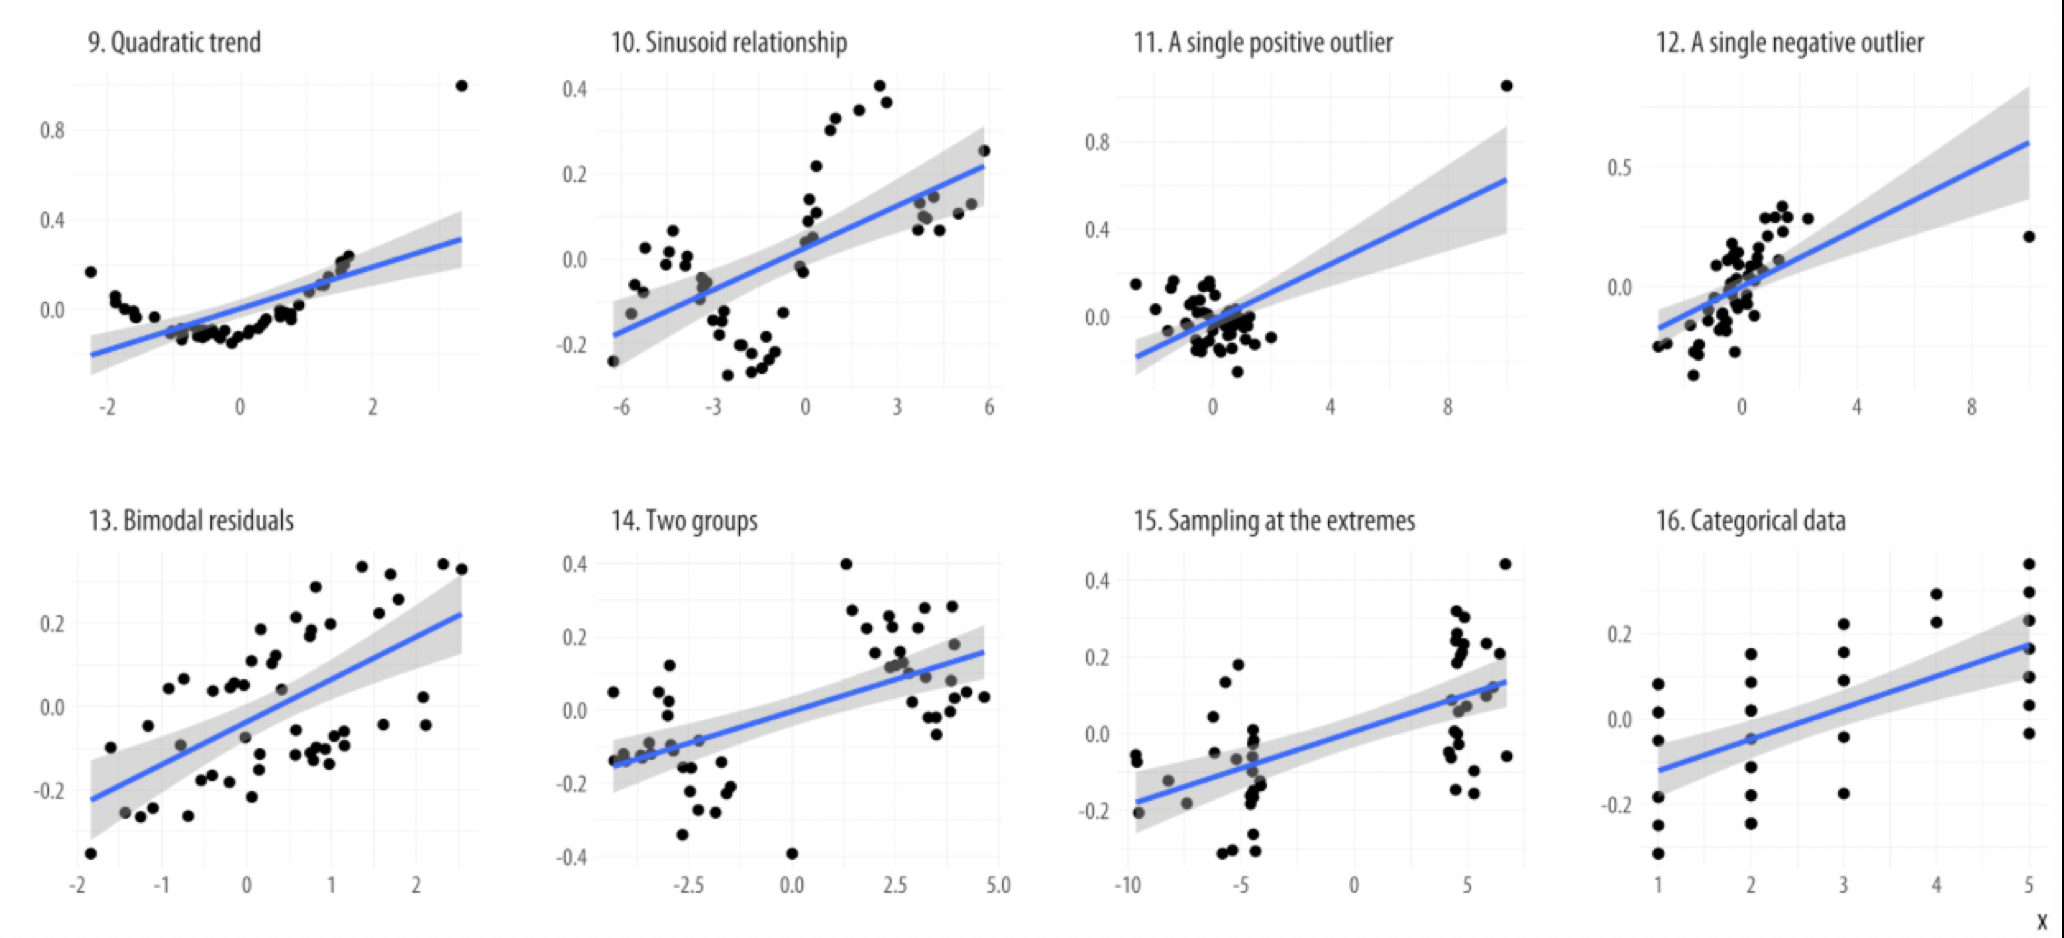
\includegraphics[width=\linewidth]{img/Shape}
\end{figure}

\end{frame}


\begin{frame}{This really matters for impact analysis}
	\begin{multicols}{2}	
		
		\begin{itemize}[<default overlay specification>]
			\item<1> In this case, for example, simply running a regression on the data would give a very wrong impression about the strength of the relationship.
			\item<1> And real data has many more than two dimensions!
		\end{itemize}
		
		\begin{figure}
			\centering
			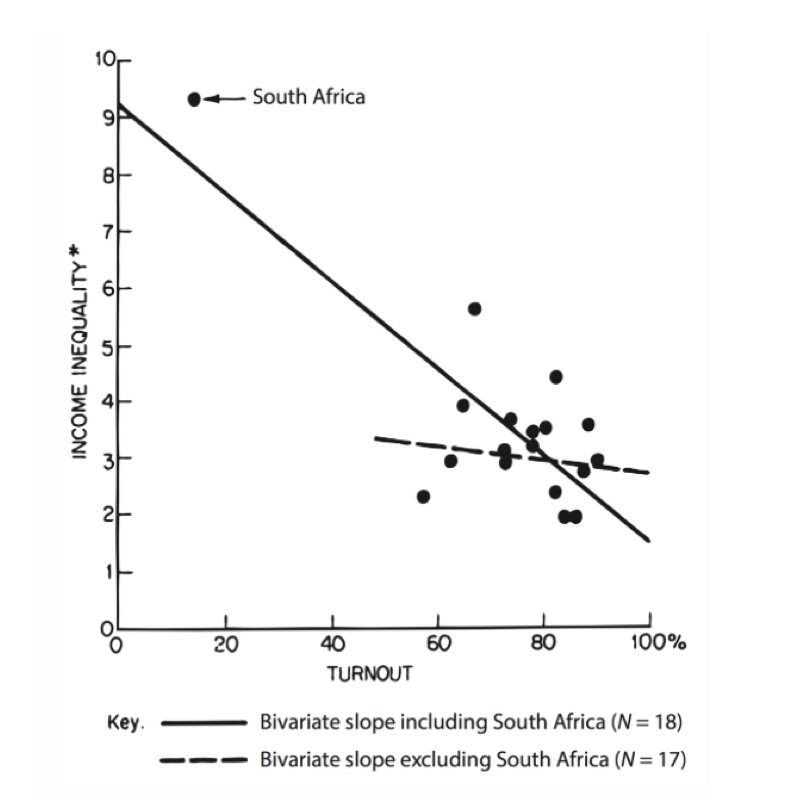
\includegraphics[width=70mm]{img/Impact}
		\end{figure}
		
	\end{multicols}
\end{frame}


\begin{frame}{Tables present a lot of data in a small space}
	
	\begin{figure}
		\centering
		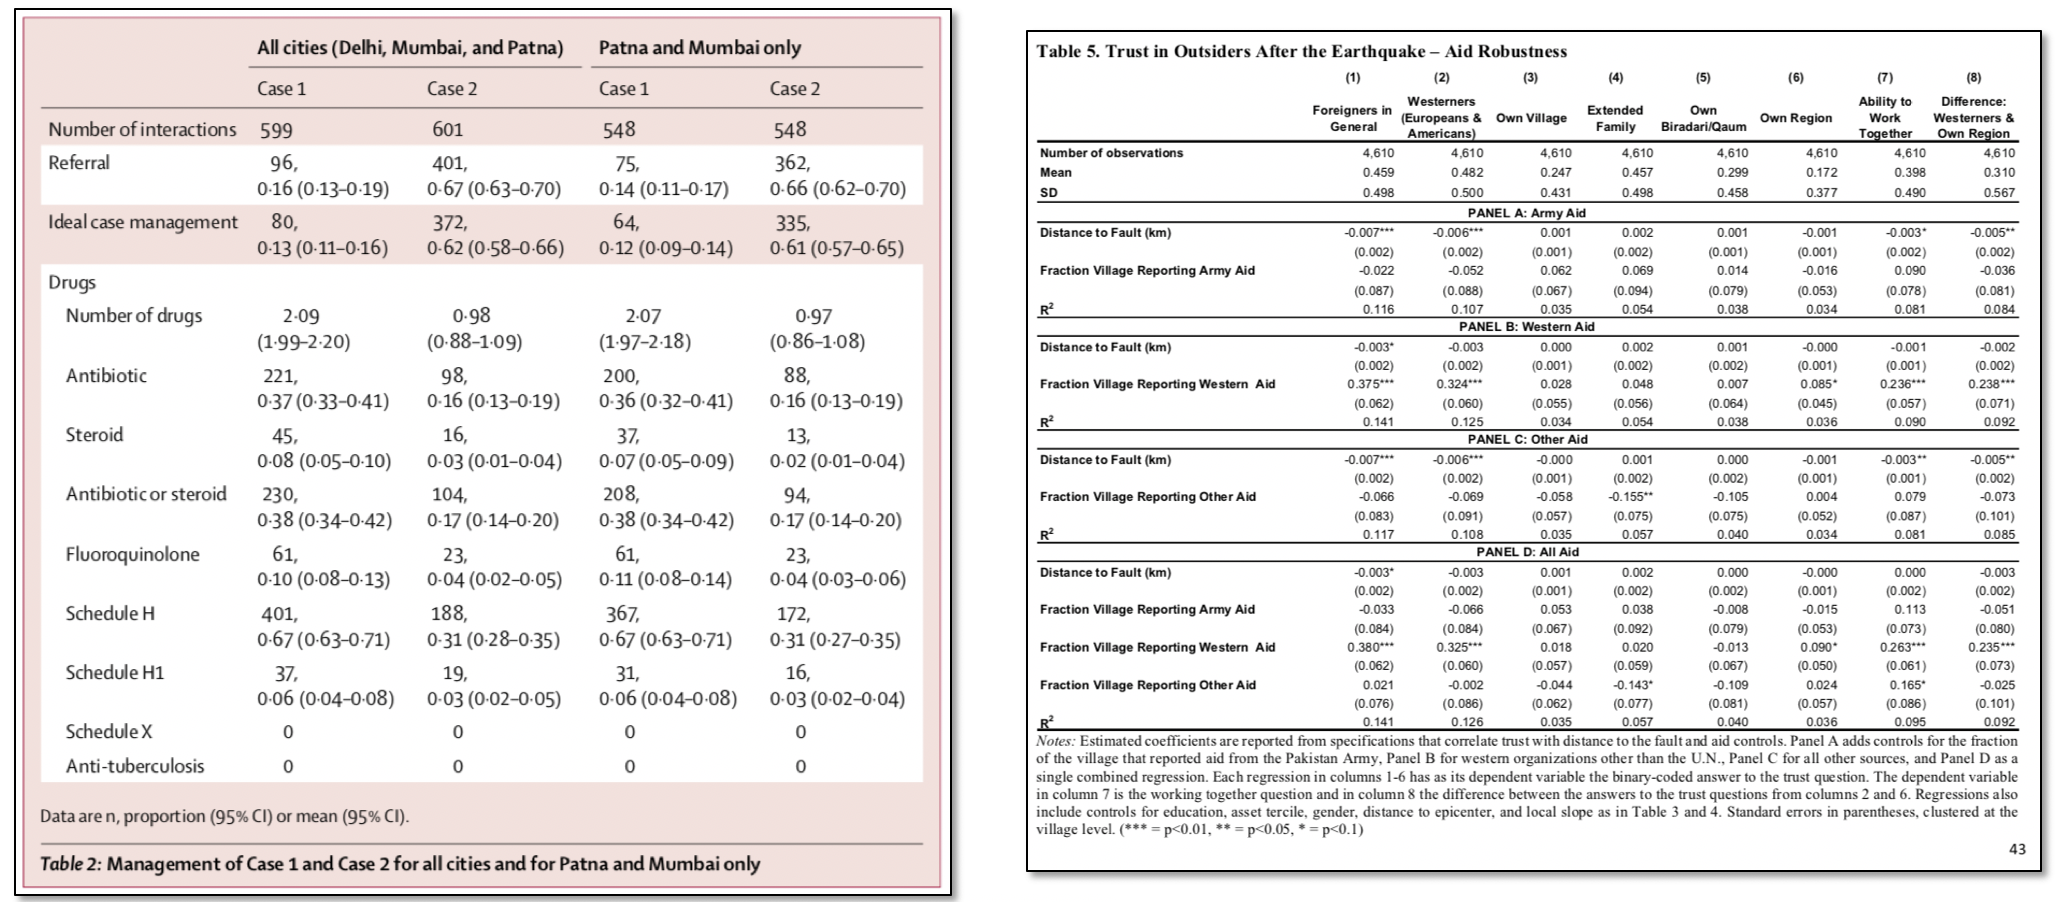
\includegraphics[width=\linewidth]{img/Table}
	\end{figure}
	
\end{frame}


\begin{frame}{Tables are important and also hard}
		
		\begin{itemize}[<default overlay specification>]
			\item<1> I will not focus on design here: putting tables together is hard enough!
			\item<1> There are several options for both Excel and LaTeX.
		\end{itemize}
		
		\begin{figure}
			\centering
			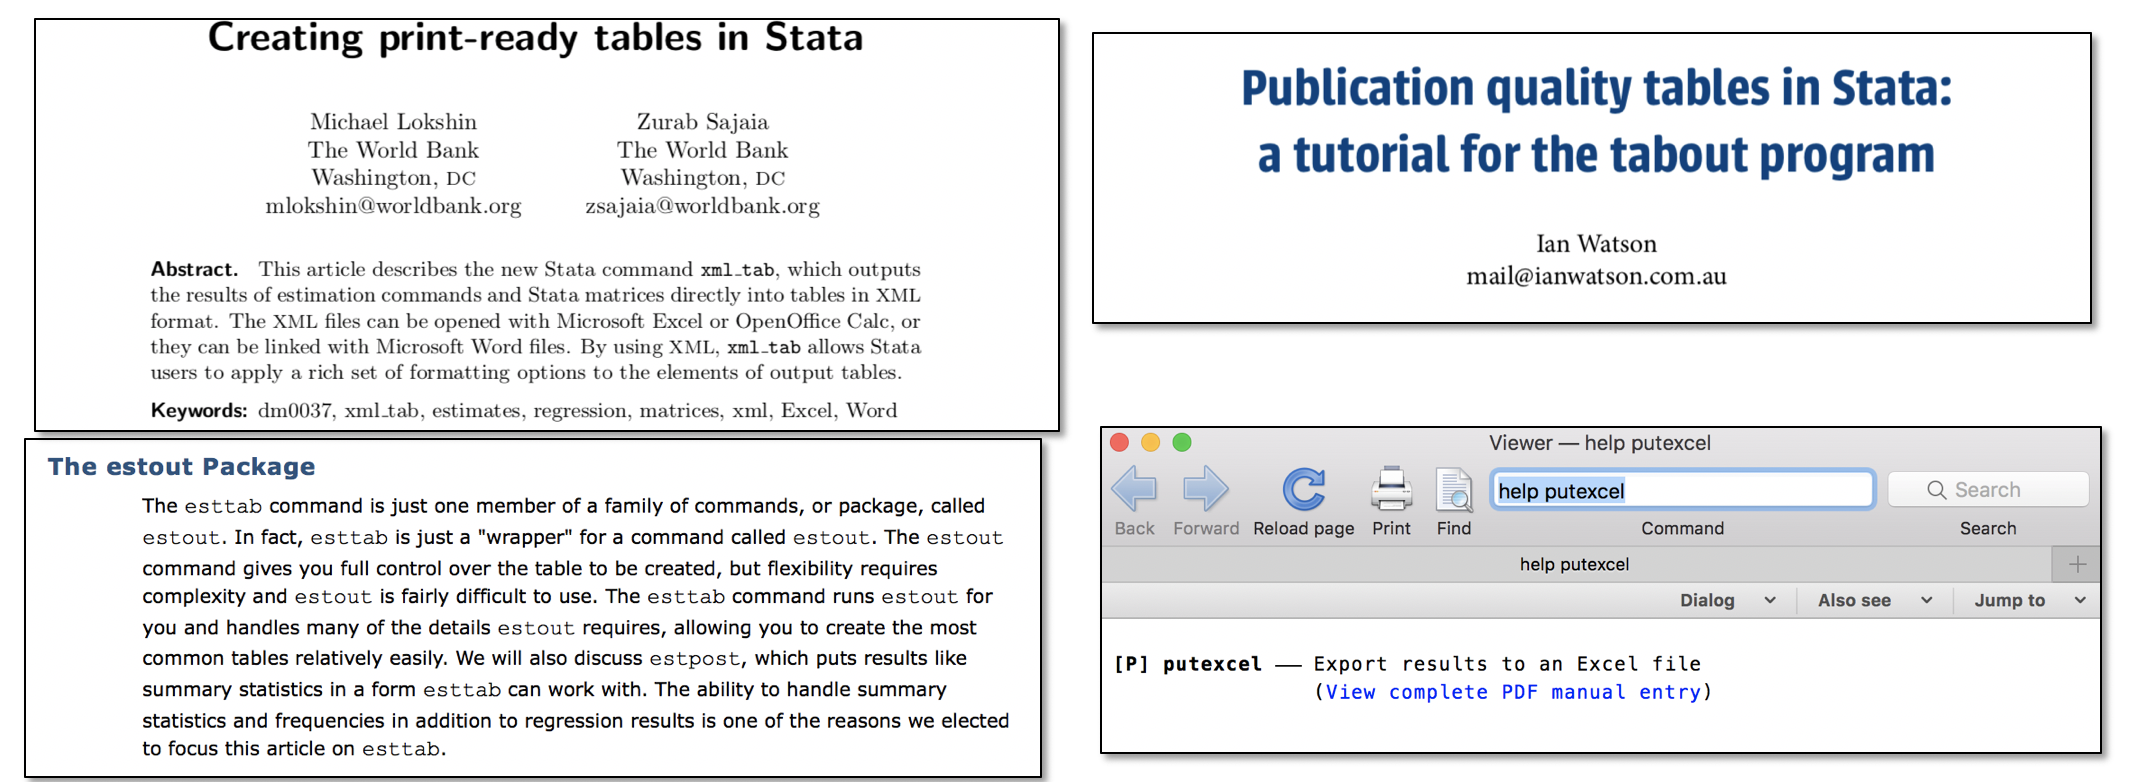
\includegraphics[width=90mm]{img/Table2}
		\end{figure}
		
\end{frame}


\begin{frame}{Process reminder: Keep “raw” files separate}
	\begin{multicols}{2}	
		
		\begin{itemize}[<default overlay specification>]
			\item<1> Each table should be created into a separate output file that says exactly what it is, and have its own section of code to re-create.
			\item<1> It’s tempting to write impressive code to make all the tables at once in one file!
			\item<1> But this makes your code less modular and readable.
		\end{itemize}
		
		\begin{figure}
			\centering
			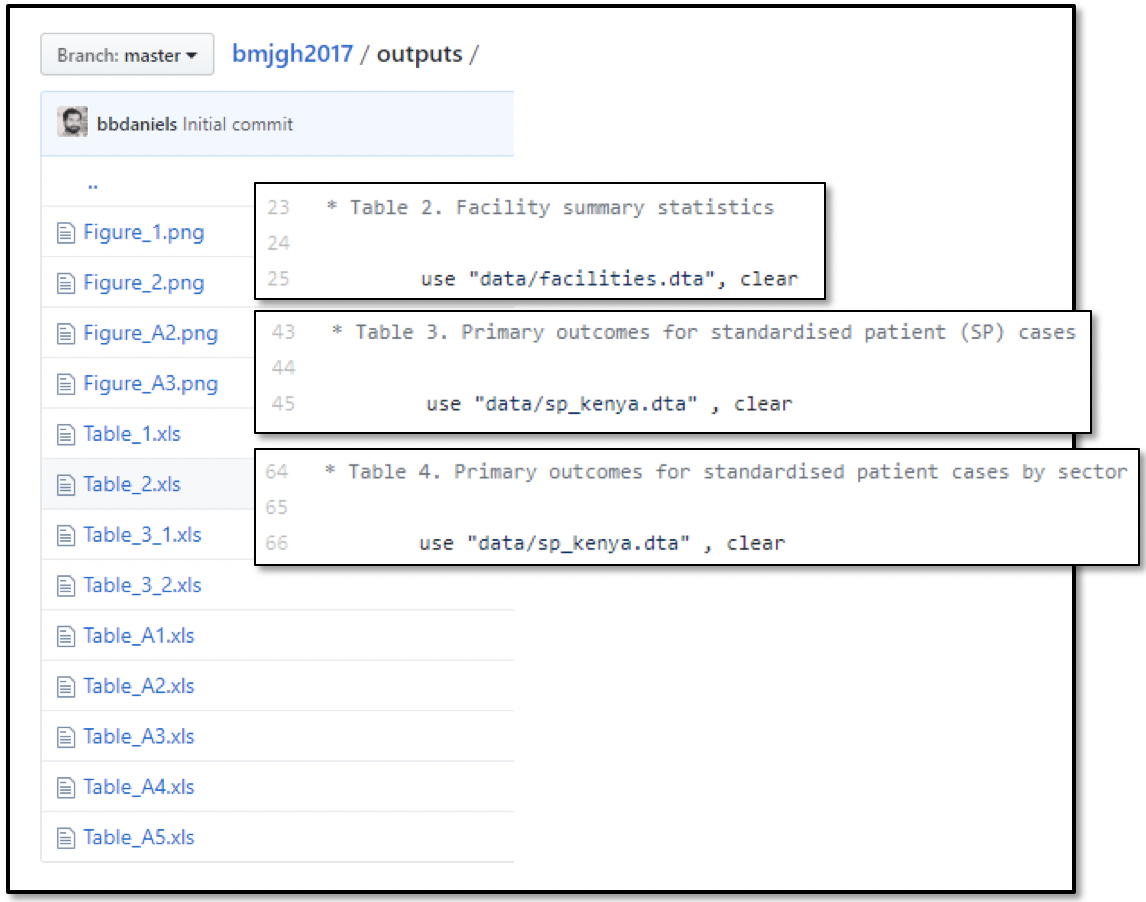
\includegraphics[width=70mm]{img/Raw}
		\end{figure}
		
	\end{multicols}
\end{frame}


\begin{frame}{Three most common types of tables}
	\begin{multicols}{2}	
		
		\begin{itemize}[<default overlay specification>]
			\item<1> \textbf{Summary statistics}.
				\newline - Show an overview of variable distributions, possible for multiple groups.
			\item<1> \textbf{Balance tests}.
				\newline - Show a direct comparison of variable means across treatment arms.
			\item<1> \textbf{Regression outputs}.
				\newline - Estimate parameters of interest like treatment effects.
		\end{itemize}
		
		\begin{figure}
			\centering
			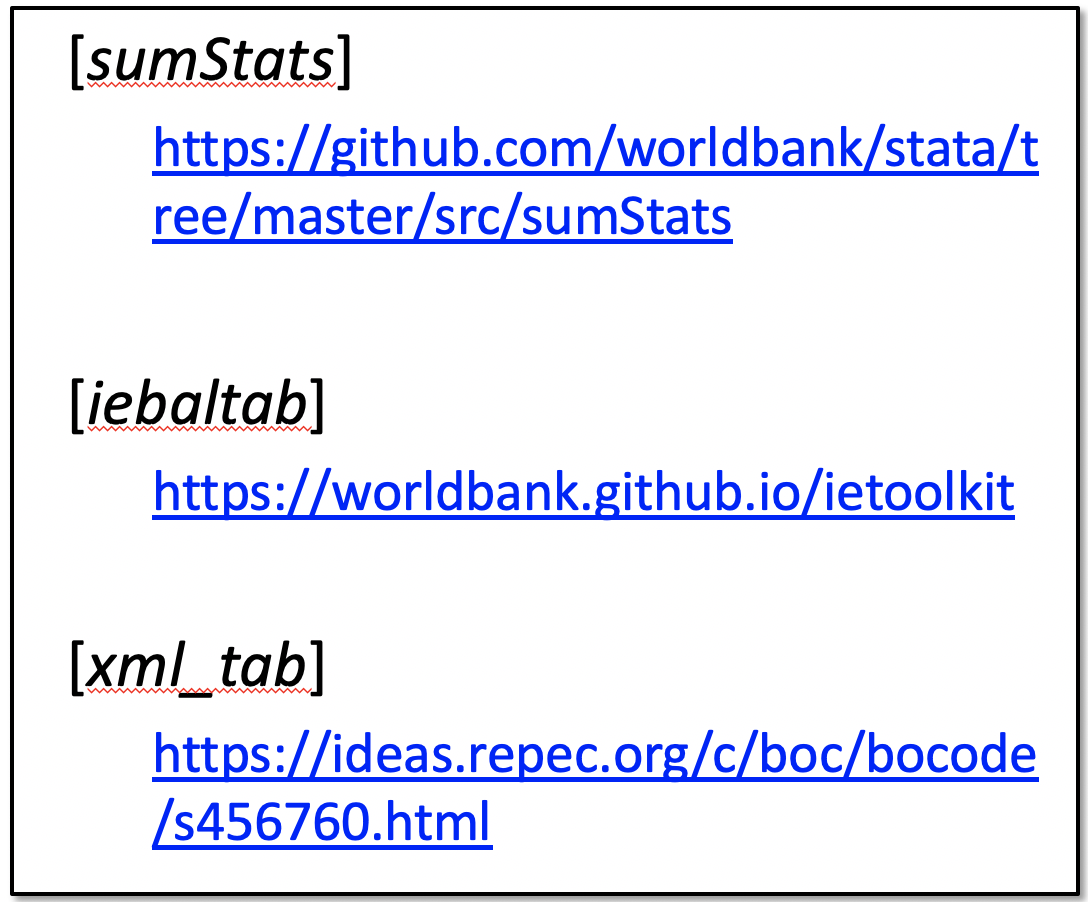
\includegraphics[width=70mm]{img/Table3}
		\end{figure}
		
	\end{multicols}
\end{frame}


\begin{frame}{Summary statistics with [sumStats]}
	\begin{multicols}{2}	
		
		\begin{itemize}[<default overlay specification>]
			\item<1> (sumStats) is a command that will output anything you can get from [tabstat].
			
			\begin{figure}
				\centering
				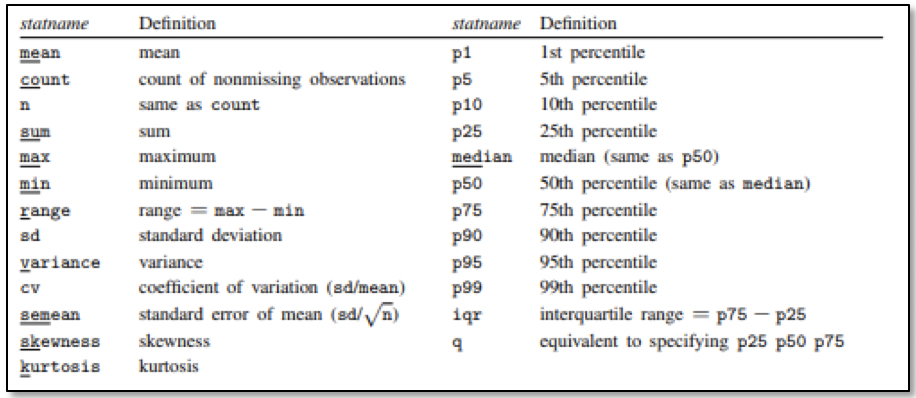
\includegraphics[width=50mm]{img/Table4}
			\end{figure}
			
			\item<1> It also allows multiple [if]-restrictions with different variable lists.
		\end{itemize}
		
		\begin{figure}
			\centering
			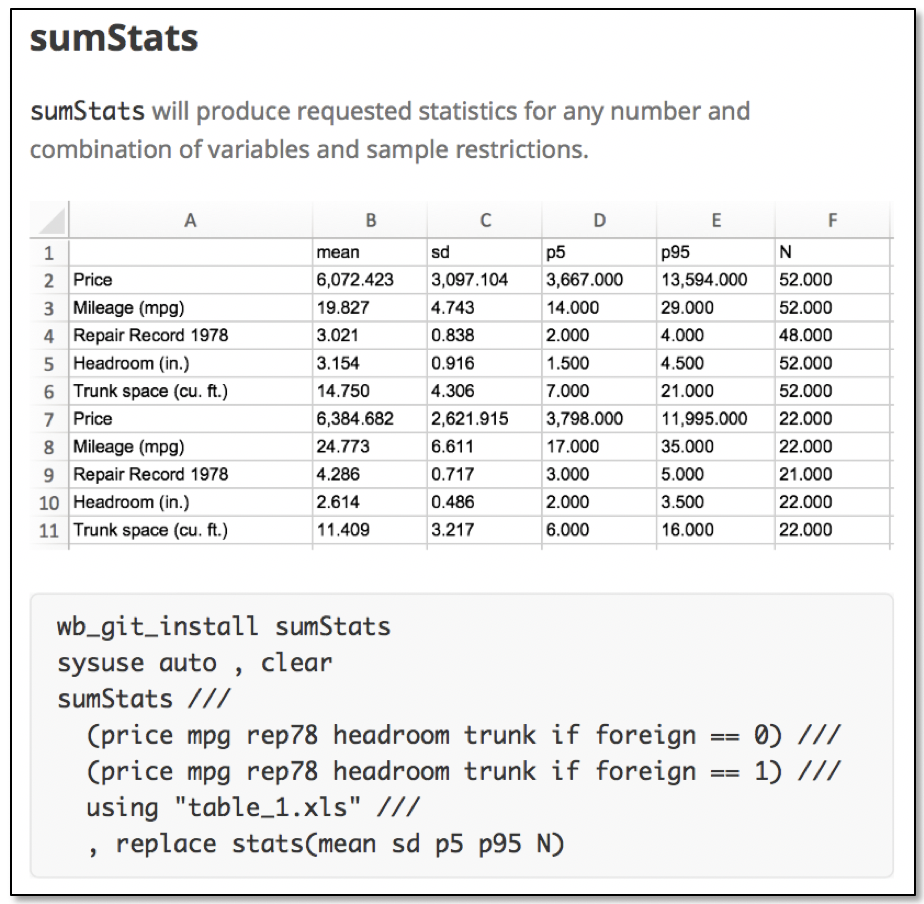
\includegraphics[width=70mm]{img/Table5}
		\end{figure}
		
	\end{multicols}
\end{frame}


\begin{frame}{Multiple levels or groups are easy}
	\begin{multicols}{2}	
		
		\begin{itemize}[<default overlay specification>]
			\item<1> Village statistics can be called with (if tag\_village == 1)
			
			\begin{figure}
				\centering
				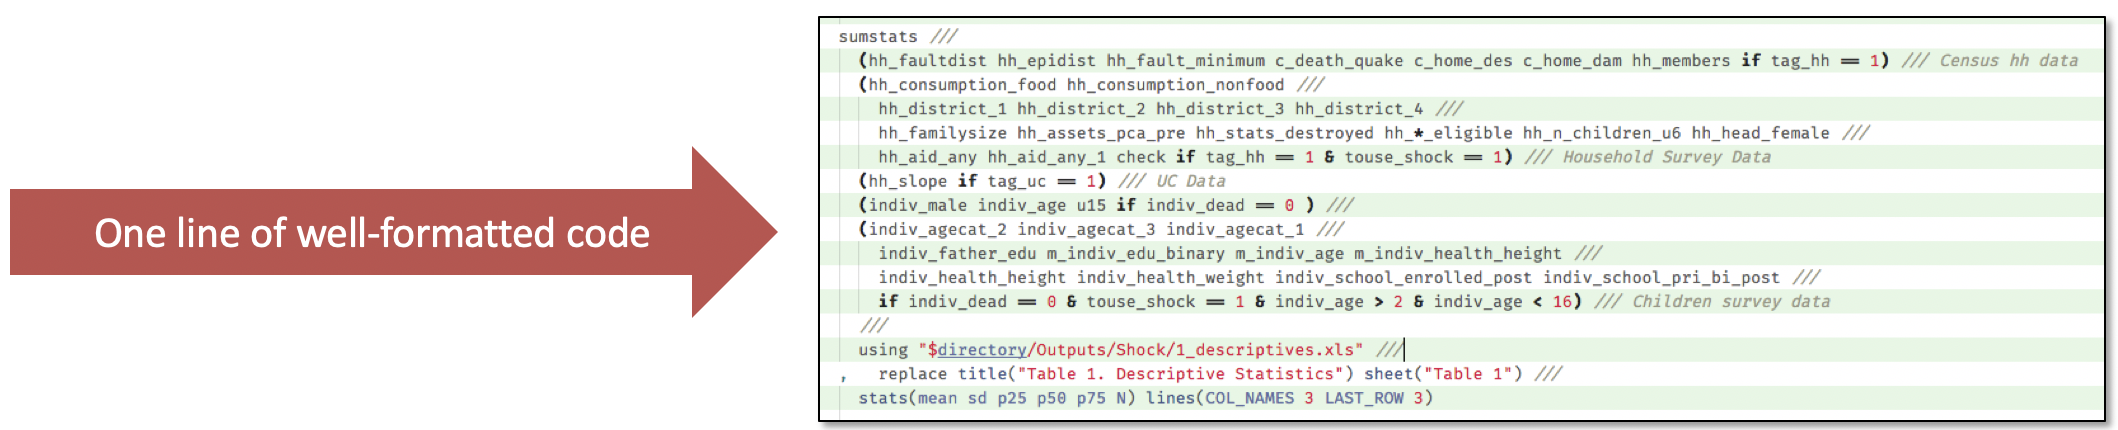
\includegraphics[width=70mm]{img/Table6}
			\end{figure}
			
			\item<1> Treatment group can be called with [if treatment == 1].
			\item<1> And so on, with only one line of code in Stata.
		\end{itemize}
		
		\begin{figure}
			\centering
			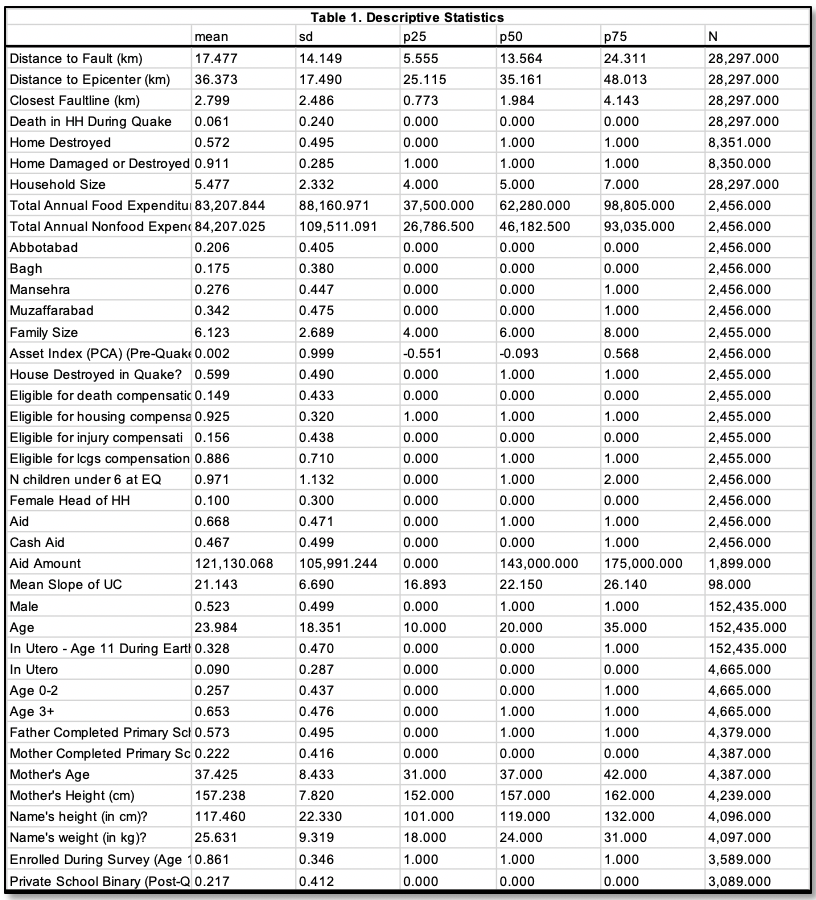
\includegraphics[width=50mm]{img/Table7}
		\end{figure}
		
	\end{multicols}
\end{frame}


\begin{frame}{Balance tables with [iebaltab]}
	\begin{multicols}{2}	
		
		\begin{itemize}[<default overlay specification>]
			\item<1> Balance tables feature in almost every impact evaluation.
			\item<1> We use balance tables to show that there was no difference between our control and treatment group in the baseline before the intervention. 
			\item<1> To us [iebaltab], list all the variables you want to test balance in, and use the option [grpvar()] to indicate which group each observation is in.
		\end{itemize}
		
		\begin{figure}
			\centering
			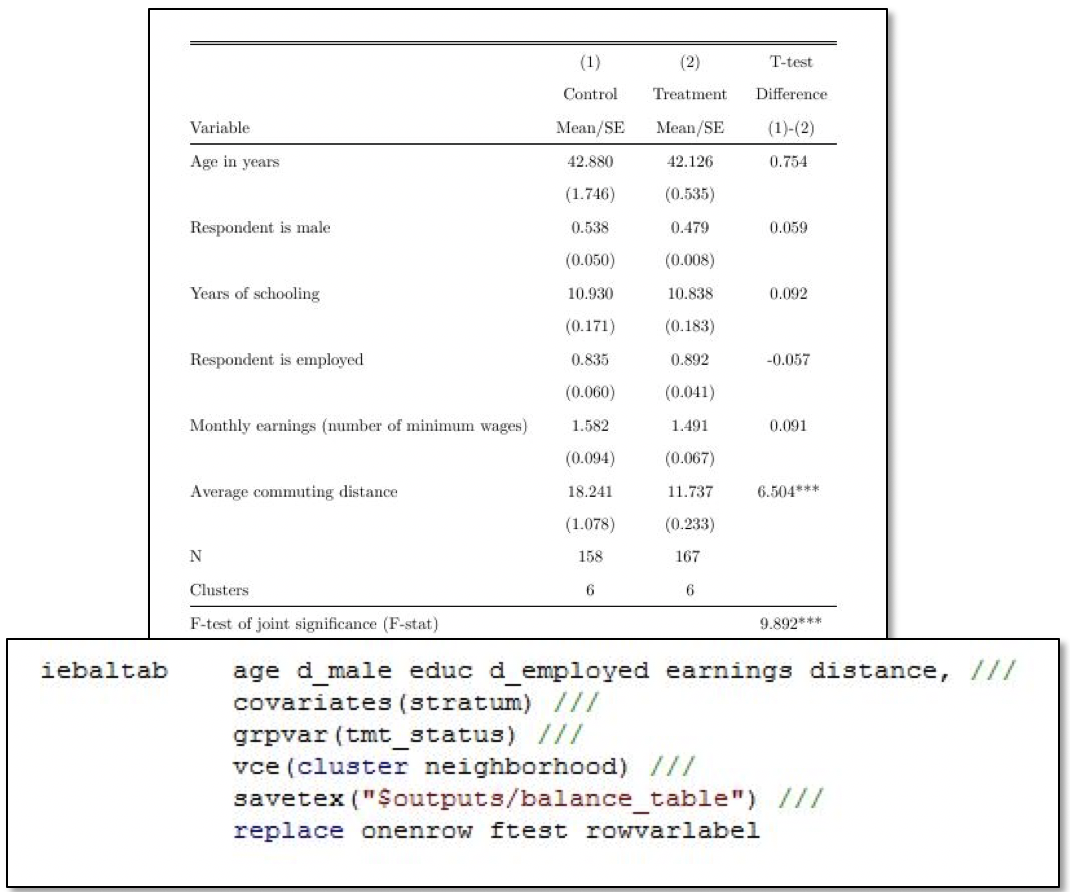
\includegraphics[width=70mm]{img/Iebaltab}
		\end{figure}
		
	\end{multicols}
\end{frame}


\begin{frame}{Balance tables with [xmltab]}
	\begin{multicols}{2}	
		
		\begin{itemize}[<default overlay specification>]
			\item<1> \textbf{Powerful regression engine:} automatically aligns regression coefficients across models.
			\item<1> \textbf{Accepts arbitrary matrices:} Very easy to hack [xmltab] into doing whatever you want. 
			\item<1> \textbf{Flexible formatting syntax:} Allows reasonable customization of decimal places, stars, etc. via Excel formatting styles.
		\end{itemize}
		
		\begin{figure}
			\centering
			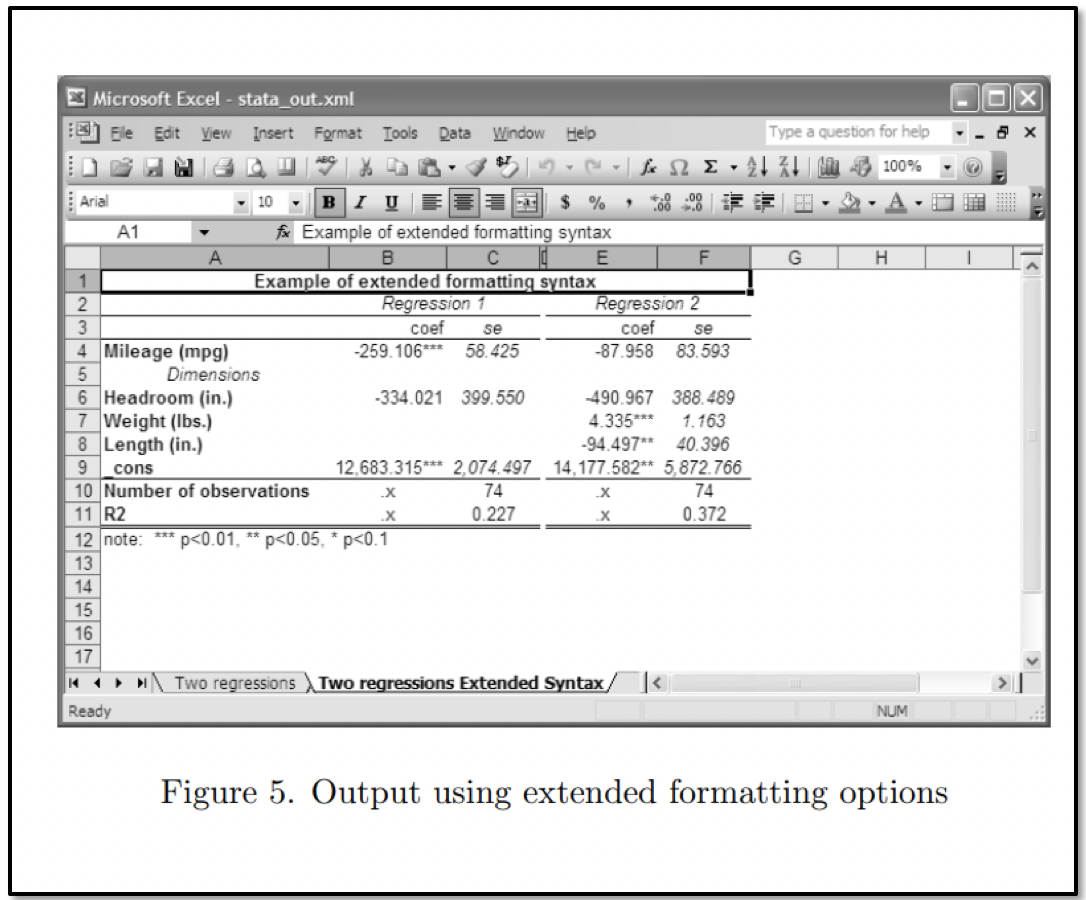
\includegraphics[width=70mm]{img/Xml_tab}
		\end{figure}
		
	\end{multicols}
\end{frame}


\begin{frame}{Regressions are automatically stacked up}
	
	\begin{figure}
		\centering
		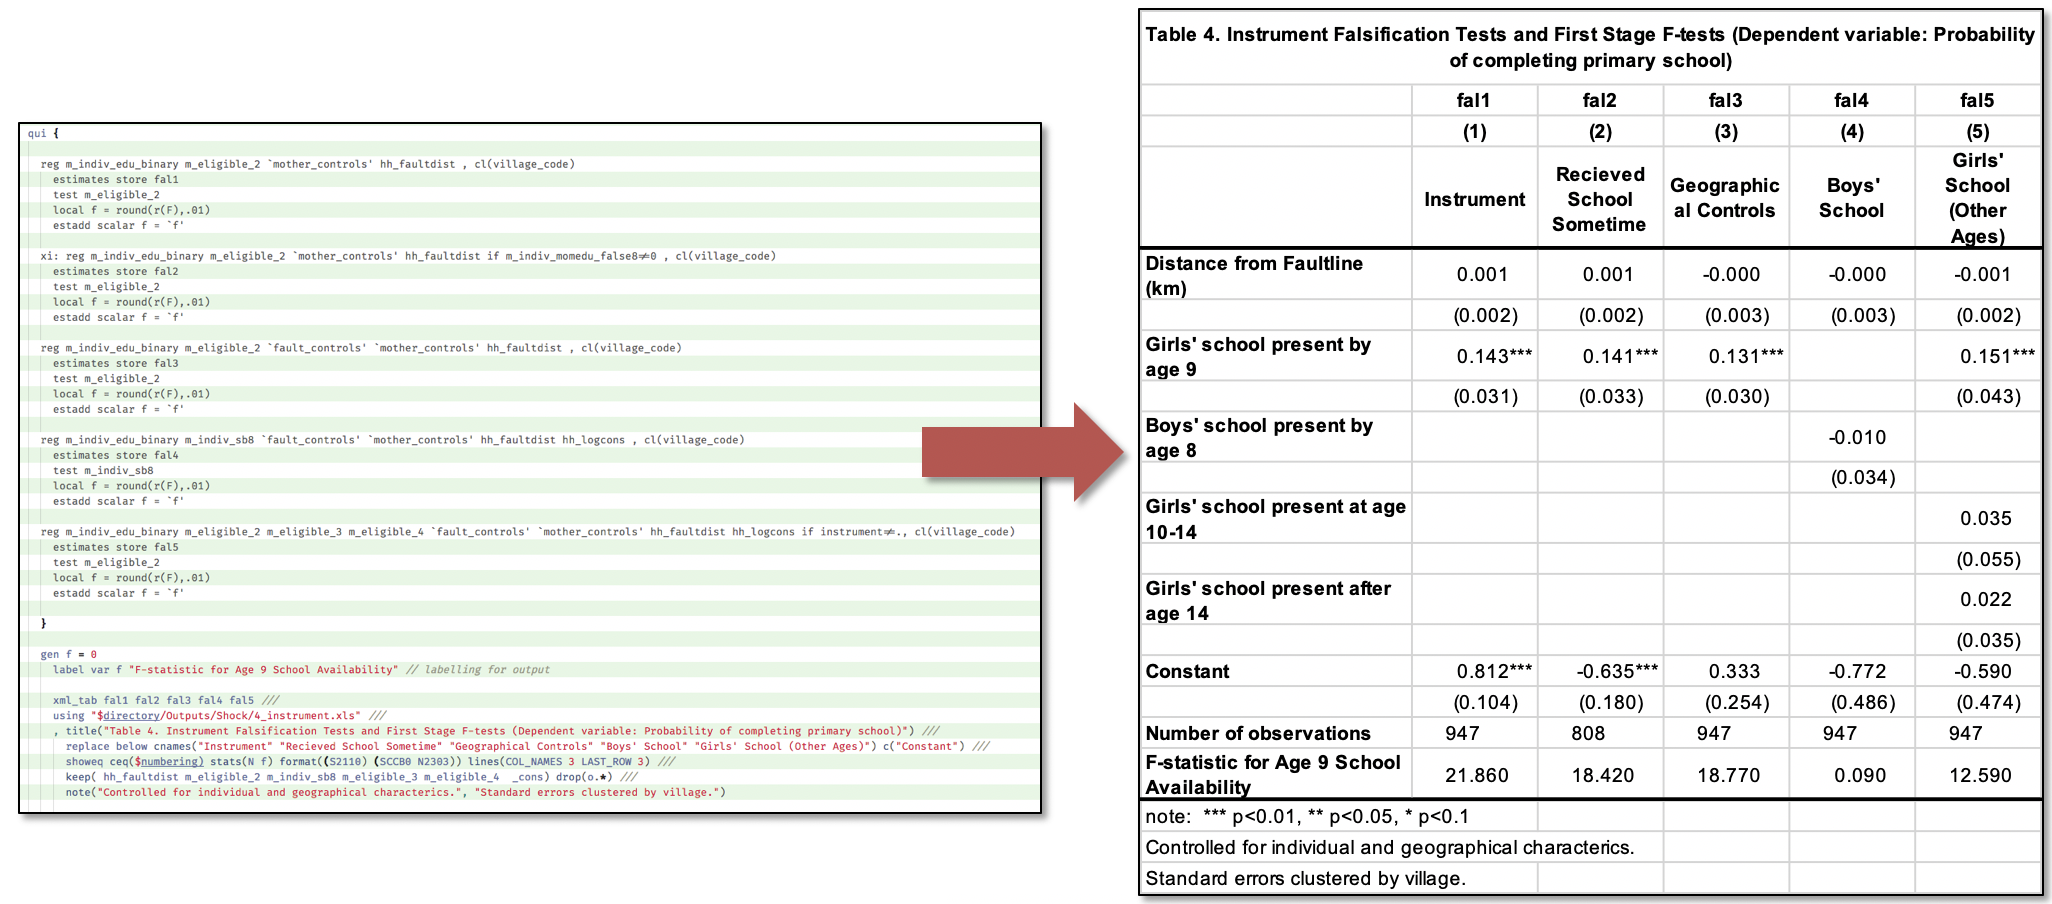
\includegraphics[width=\linewidth]{img/Regressions2}
	\end{figure}
	
\end{frame}


\begin{frame}{Helpful checklist before sending tables to PI}
	\begin{multicols}{2}	
		
		\begin{itemize}[<default overlay specification>]
			\item<1> Does the number of observations for each regression or summary statistic make sense?
			\item<1> Do the magnitude and sign of each coefficient/summary statistic seem reasonable?
			\item<1> Did you delete the constant term and add the control mean in the regression table?
			\item<1> Did you check for joint significance of your covariates?
			\item<1> Did you label the dependent variables/columns?
			\item<1> Did you label the covariates/rows?
			\item<1> Did you add a title?
			\item<1> Is it clear what the estimation procedure is (e.g. regression vs. probit)?
			\item<1> Are the column widths the right size so as not to cut off text?
			\item<1> Is the bordering consistent with your other tables?
			\item<1> Are the numbers rounded to an appropriate level, so you don’t display too many decimal places?
			\item<1> Do the notes to the table clearly indicate how standard errors have been estimated, and what control variables if any have been included but not shown?
		\end{itemize}
		
	\end{multicols}
\end{frame}

%%%%%%%%%%%%%%%%%%%%%%%%%%%%%%%%%%%%%%%%%%% Final thougts section
\begin{frame}{Conclusion}

Thank You!

\vspace{20mm}
For more information or further questions please contact:
\newline Benjamin Daniels  (\url{bdaniels@worldbank.org}) 

\end{frame}

%%%%%%%%%%%%%%%%%%%%%%%%%%%%%%%%%%%%%%%%%%% The End
\sectionpic{The End}{img/section_slide}






\end{document} 